%% ---------------------------------------------------------------------------
%%  Springer LNCS Proceedings manuscript (llncs class)
%%  Adapted from the samplepaper.tex LLNCS template.
%%
%%  Compile with:
%%      pdflatex main && bibtex main && pdflatex main && pdflatex main
%% ---------------------------------------------------------------------------
\documentclass[runningheads]{llncs}

\usepackage[T1]{fontenc}
% The LLNCS template uses the newtx Times fonts; fall back to Times
% (mathptmx) on installations where newtxtext/newtxmath are unavailable.
\IfFileExists{newtxtext.sty}{%
  \usepackage{newtxtext}
  \usepackage[varvw]{newtxmath}%
}{%
  \usepackage{mathptmx}%
}
\usepackage{microtype}
\setlength{\emergencystretch}{2em}
\usepackage{amsmath,amssymb}
\usepackage{graphicx}
\usepackage{booktabs}
\usepackage{float}
\usepackage{tikz}
\usepackage{pgfplots}
\pgfplotsset{compat=1.17}
\usetikzlibrary{arrows.meta,positioning,shapes.geometric}
\usepackage[hidelinks]{hyperref}

\begin{document}

\title{Securing Lattice-Based Secret Sharing with Steganography: A Post-Quantum
Threshold Construction and Empirical Evaluation}
%
\titlerunning{Lattice-Based Secret Sharing with Steganography}
%
\author{TADMON-YAYA Franklin Lenny\inst{1}}
%
\authorrunning{F. L. TADMON-YAYA}
%
\institute{Department of Computer Science, University of Yaounde I, Yaounde,
Cameroon\\
\email{tadmonyayafranklin@gmail.com}}
%
\maketitle

\begin{abstract}
Threshold secret sharing underpins distributed trust, yet most deployed
schemes were designed against classical adversaries. The anticipated maturity
of large-scale quantum computers, and Shor's polynomial-time algorithm for the
hidden-subgroup problems underlying RSA and elliptic-curve cryptography,
motivate re-examining threshold constructions through a post-quantum lens.
This work presents and evaluates a framework that (i) performs threshold secret
sharing on a lattice foundation by combining Regev-style Learning With Errors
(LWE) encryption with Shamir polynomial sharing over the prime field
$\mathbb{Z}_q$, and (ii) conceals each participant's share in digital cover
media using spatial least-significant-bit (LSB), frequency-domain discrete
cosine transform (DCT), and audio pulse-code-modulation (PCM) steganography. A
Java reference implementation was ported to Android. On standard test imagery
(Baboon, Cat, Lenna, Pepper) and a synthetic cover, LSB embedding achieved peak
signal-to-noise ratios (PSNR) of $81.6$--$88.5~\mathrm{dB}$ (MSE
$\sim\!10^{-4}$), whereas DCT achieved $36.8$--$38.8~\mathrm{dB}$ (MSE
$8.7$--$13.6$); audio LSB over 16-bit PCM averaged MSE
$\sim\!8.3\times10^{-3}$. Reconstruction was exact for every threshold tested
($2 \le k \le 10$) and correctly refused for $k-1$ shares. These results
indicate that a post-quantum, LWE-based threshold scheme can be coupled with
high-fidelity steganographic transport without loss of secret integrity,
although the parameter set is demonstrative and no formal reduction is claimed.

\keywords{post-quantum cryptography \and learning with errors \and threshold
secret sharing \and image steganography \and discrete cosine transform.}
\end{abstract}

%% ===========================================================================
\section{Introduction}
\label{sec:intro}
%% ===========================================================================

\subsection{Background and Context}

Secret sharing allows a dealer to distribute a secret among $n$ participants
such that only authorized coalitions can reconstruct it. Since the seminal,
independent proposals of Shamir \cite{shamir1979} and Blakley
\cite{blakley1979}, threshold schemes have become foundational to threshold
signatures, secure multiparty computation, distributed key management, and
hardware security modules. Shamir's scheme remains canonical because it is not
only efficient but \emph{information-theoretically secure}: fewer than $k$
shares reveal no information about the secret, irrespective of computational
assumptions.

This last property is frequently invoked to argue that secret sharing is
already resistant to quantum adversaries. That argument is incomplete in
practice. Real threshold deployments do not distribute bare field elements;
they distribute shares through transport channels, storage media, and
key-wrapping layers that depend on public-key primitives vulnerable to Shor's
algorithm \cite{shor1994}. Moreover, the growing adoption of lattice-based
standards---exemplified by the NIST post-quantum selections, notably ML-KEM
(CRYSTALS-Kyber) and ML-DSA (CRYSTALS-Dilithium) \cite{nist2024,avanzi2020,ducas2018}---establishes
Learning With Errors (LWE) and its ring variants as the de facto post-quantum
substrate \cite{regev2005,peikert2009,micciancio2009}. It is therefore natural
to ask how threshold secret sharing should be reconstructed on lattice
assumptions, and how the resulting shares can be transported covertly.

In parallel, steganography---the art of embedding messages within innocuous
cover objects---offers a complementary protection layer
\cite{simmons1984,cachin1998,provos2003,fridrich2009}. By hiding a share
inside a cover image or audio stream, the very \emph{existence} of the share
can be denied, an objective distinct from, and often stronger than, the
confidentiality offered by encryption alone. Classical LSB substitution
\cite{bender1996,chan2004} and frequency-domain methods such as DCT-based and
F5 embedding \cite{westfeld2001} are well studied, but their integration with
post-quantum threshold primitives has received comparatively little attention.

\subsection{The Research Gap}

The literature contains rich, separate streams on (a) lattice-based encryption
\cite{regev2005,gentry2008}, (b) threshold and distributed decryption for
lattice cryptosystems \cite{bendlin2010,desmedt1994,gemmell1997}, and (c)
image and audio steganography
\cite{chan2004,westfeld2001,johnson1998,petitcolas1999}. What is
comparatively under-explored is an \emph{end-to-end} treatment that answers two
coupled questions: Can the shares of a post-quantum threshold scheme be
embedded in cover media without compromising exact reconstruction? And what is
the measurable fidelity cost of doing so under different embedding domains?
Prior prototype work on combinatorial (``matrix-counting'') secret sharing has
demonstrated the steganographic pipeline's mechanics but rests on a
non-standard, non-post-quantum sharing rule. The research gap addressed here is
the \emph{absence of an empirically characterized pipeline that replaces a
counting-based sharing primitive with a lattice-based one while
preserving---and quantifying---steganographic performance}.

\subsection{Hypothesis and Objectives}

We hypothesize that an LWE-based threshold sharing construction, in which the
lattice secret key is distributed via Shamir sharing over $\mathbb{Z}_q$ and
each participant's share is embedded into a cover medium, reconstructs the
secret exactly whenever at least $k$ shares are available and refuses
reconstruction otherwise, while maintaining cover-media fidelity consistent
with the embedding domain. Accordingly, the objectives are:

\begin{enumerate}
  \item To formulate a post-quantum threshold secret sharing construction that
        composes Regev-style LWE encryption with Shamir sharing of the LWE
        secret key over $\mathbb{Z}_q$.
  \item To design a serialization that represents a share as a fixed-length bit
        string suitable for generic steganographic embedding.
  \item To implement the construction and three embedding channels (image LSB,
        image DCT, audio PCM LSB) in a reproducible reference system.
  \item To measure reconstruction correctness across thresholds and the
        fidelity cost (MSE/PSNR) on standard imagery and synthetic audio.
\end{enumerate}

%% ===========================================================================
\section{Materials and Methods}
\label{sec:methods}
%% ===========================================================================

\subsection{Ethics Statement}

This study did not involve human participants, personally identifiable
information, or animal subjects. All image datasets are standard, publicly
available test images, and all audio material was generated synthetically. No
ethical approval was required.

\subsection{Experimental Design}

The study followed a single-factor, multi-condition experimental design with
exact reconstruction as the dependent correctness measure and cover fidelity as
the dependent quality measure. Three factors were varied: (i) the
reconstruction threshold $k$ over the range $2 \le k \le 10$ with a fixed
participant count $n = 10$; (ii) the embedding domain (spatial LSB, frequency
DCT, audio LSB); and (iii) the cover source (four standard images, one
synthetic image, and a synthetic WAV). For each condition the secret was
reconstructed from exactly $k$ shares (expected: success) and from $k-1$ shares
(expected: refusal). A non-binary secret (a bank-code string) was additionally
processed block-wise to test generalization to arbitrary byte content.

\subsection{Materials and System Specification}

The reference implementation comprises a Java~17 code base and an Android port.
The cryptographic core is parameterized by a prime modulus $q = 12{,}289$, a
lattice dimension $n = 8$, and $m = 32$ LWE samples. The LWE secret $\mathbf{s}$
is a binary vector. Errors are drawn uniformly from $\{-1,0,1\}$. A serialized
share occupies $128$ bits (a $16$-bit participant index and eight $14$-bit
field elements). The illustrative secret used throughout is the six-bit string
\texttt{100100} (hexadecimal \texttt{24}), chosen to mirror the worked example
of prior counting-based prototypes. Software was executed on a commodity
x86-64 workstation; the Android port used \texttt{android.graphics.Bitmap} in
place of \texttt{java.awt.image.BufferedImage}.

\paragraph{LWE key generation and encryption.}
The dealer samples a secret vector $\mathbf{s} \gets \{0,1\}^n$, a public
matrix $\mathbf{A} \in \mathbb{Z}_q^{m \times n}$, and a small error
$\mathbf{e}$, and publishes
\begin{equation}
  \mathbf{b} = \mathbf{A}\,\mathbf{s} + \mathbf{e} \pmod{q}.
  \label{eq:key}
\end{equation}
Each secret bit $\mu \in \{0,1\}$ is encrypted with fresh randomness
$\mathbf{x} \in \{0,1\}^m$ and error $e'$:
\begin{equation}
  \mathbf{u} = \mathbf{A}^{\!\top}\mathbf{x} \pmod{q},
  \qquad
  c = \mathbf{b}^{\!\top}\mathbf{x} + e' + \mu\,\lfloor q/2 \rfloor \pmod{q}.
  \label{eq:enc}
\end{equation}

\paragraph{Threshold key distribution.}
The LWE secret key is shared with Shamir's scheme over the field
$\mathbb{Z}_q$. For each coordinate $j \in \{1,\dots,n\}$ the dealer samples a
degree-$(k-1)$ polynomial
\begin{equation}
  f_j(X) = s_j + a_{j,1}X + \dots + a_{j,k-1}X^{k-1} \pmod{q},
  \label{eq:poly}
\end{equation}
and issues to participant $i$ the share
$\bigl(i,\ f_1(i),\ \dots,\ f_n(i)\bigr)$. Reconstruction with $k$ shares
interpolates each coordinate at the origin,
\begin{equation}
  s_j = \sum_i y_{i,j}\,L_i(0),
  \qquad
  L_i(0) = \prod_{l \neq i} \frac{-x_l}{x_i - x_l} \pmod{q},
  \label{eq:lagrange}
\end{equation}
and decryption recovers each bit by rounding the centered residual
\begin{equation}
  \mu = 1 \quad\text{if}\quad
  \bigl|\,(c - \langle \mathbf{u}, \mathbf{s}\rangle) \bmod q\,\bigr|
  > \lfloor q/4 \rfloor, \quad\text{else}\quad 0.
  \label{eq:dec}
\end{equation}
Correctness follows because the residual equals
$\langle \mathbf{e}, \mathbf{x}\rangle + e' + \mu\lfloor q/2\rfloor$; since
$|\langle \mathbf{e}, \mathbf{x}\rangle + e'| \le m + 1 = 33 \ll \lfloor q/4
\rfloor = 3{,}072$, the rounding threshold separates the two symbols with a
wide margin.

\paragraph{Steganographic channels.}
Spatial LSB embedding writes each share bit into the least significant bit of
the green channel in a key-permuted pixel order and prepends a $32$-bit length
header for blind extraction. DCT embedding partitions the green channel into
non-overlapping $8\times8$ blocks and sets a single mid-frequency coefficient
to $+\Delta$ (bit~$1$) or $-\Delta$ (bit~$0$), $\Delta = 40$, reading the sign
at extraction. Audio embedding applies LSB substitution to 16-bit PCM samples
of a RIFF/WAVE stream. Figure~\ref{fig:pipeline} summarizes the end-to-end
pipeline.

\begin{figure}[t]
\centering
\resizebox{\textwidth}{!}{%
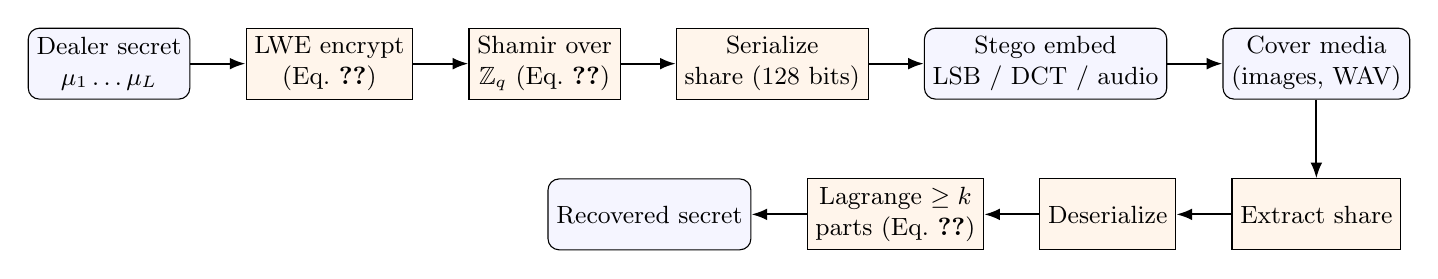
\begin{tikzpicture}[
  node distance=6mm and 7mm,
  every node/.style={font=\small},
  box/.style={draw, rounded corners, align=center, minimum height=9mm,
              inner sep=3pt, fill=blue!4},
  op/.style={draw, align=center, minimum height=9mm, inner sep=3pt,
             fill=orange!8},
  ar/.style={-{Latex[length=2mm]}, thick}
]
\node[box] (secret) {Dealer secret\\$\mu_1\dots\mu_L$};
\node[op, right=of secret] (enc) {LWE encrypt\\(Eq.~\ref{eq:enc})};
\node[op, right=of enc] (shamir) {Shamir over\\$\mathbb{Z}_q$ (Eq.~\ref{eq:poly})};
\node[op, right=of shamir] (ser) {Serialize\\share ($128$ bits)};
\node[box, right=of ser] (stego) {Stego embed\\LSB / DCT / audio};
\node[box, right=of stego] (media) {Cover media\\(images, WAV)};

\draw[ar] (secret) -- (enc);
\draw[ar] (enc) -- (shamir);
\draw[ar] (shamir) -- (ser);
\draw[ar] (ser) -- (stego);
\draw[ar] (stego) -- (media);

\node[op, below=10mm of media] (ext) {Extract share};
\node[op, left=of ext] (deser) {Deserialize};
\node[op, left=of deser] (rec) {Lagrange $\ge k$\\parts (Eq.~\ref{eq:lagrange})};
\node[box, left=of rec] (plain) {Recovered secret};

\draw[ar] (media) -- (ext);
\draw[ar] (ext) -- (deser);
\draw[ar] (deser) -- (rec);
\draw[ar] (rec) -- (plain);
\end{tikzpicture}}
\Description{End-to-end pipeline diagram: LWE encryption, Shamir sharing over
$\mathbb{Z}_q$, share serialization, steganographic embedding, and the reverse
reconstruction path.}
\caption{End-to-end pipeline: LWE encryption, Shamir sharing over
$\mathbb{Z}_q$, share serialization, steganographic embedding, and the reverse
reconstruction path.}
\label{fig:pipeline}
\end{figure}

\subsection{Data and Statistical Analysis}

Four standard images were used: Baboon ($515\times512$), Cat ($483\times395$),
Lenna ($512\times512$), and Pepper ($512\times384$); a $256\times256$
synthetic gradient served as a default cover. Audio tests used a one-second,
$8$~kHz, mono, 16-bit sinusoidal WAV. Fidelity was quantified by the mean
squared error (MSE) and peak signal-to-noise ratio (PSNR) over the three RGB
channels,
\begin{equation}
  \mathrm{MSE} = \frac{1}{3WH}\sum (P - P')^2,
  \qquad
  \mathrm{PSNR} = 10\log_{10}\!\frac{255^2}{\mathrm{MSE}}.
  \label{eq:metrics}
\end{equation}
MSE and PSNR are deterministic functions of the cover and stego media, so no
inferential statistics were required; results are reported as exact values.
Reconstruction correctness was binary (exact string match). The four standard
covers are shown in Figure~\ref{fig:covers}.

\begin{figure}[H]
\centering
\begin{tabular}{cc}
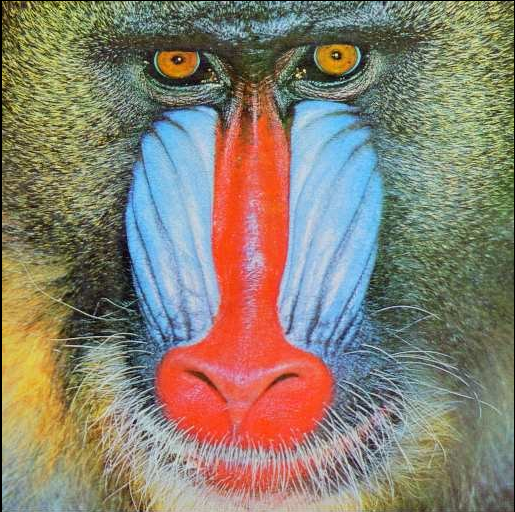
\includegraphics[width=0.40\textwidth]{images/baboon.png} &
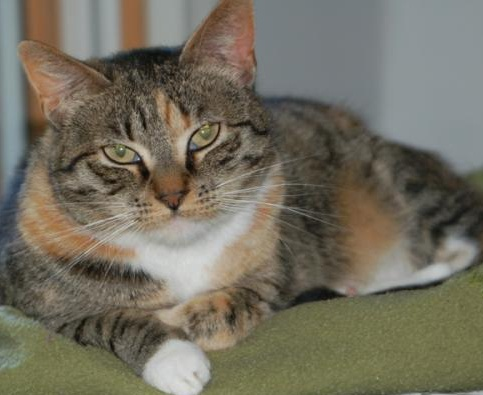
\includegraphics[width=0.40\textwidth]{images/cat.jpg}\\[2pt]
{\small (a) Baboon ($515\times512$)} & {\small (b) Cat ($483\times395$)}\\[8pt]
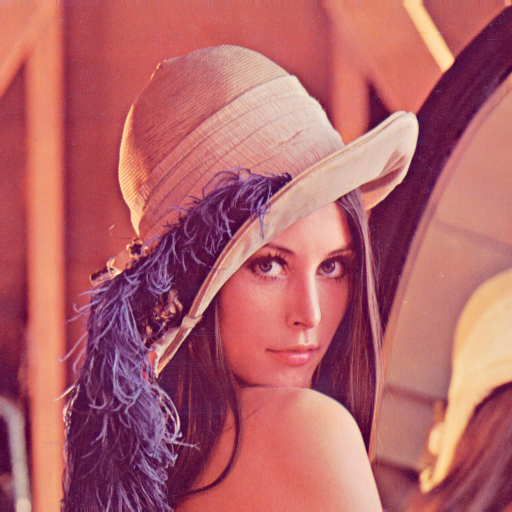
\includegraphics[width=0.40\textwidth]{images/lenna.png} &
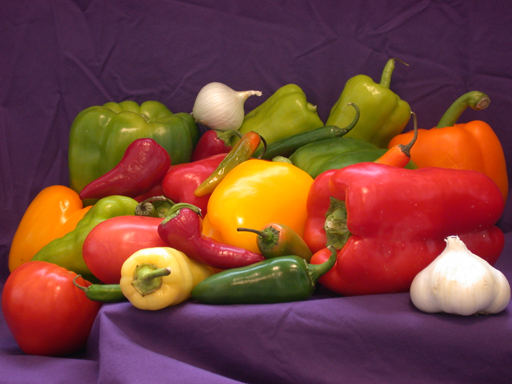
\includegraphics[width=0.40\textwidth]{images/pepper.png}\\[2pt]
{\small (c) Lenna ($512\times512$)} & {\small (d) Pepper ($512\times384$)}\\
\end{tabular}
\Description{Four standard test images used as steganographic covers: Baboon,
Cat, Lenna, and Pepper.}
\caption{Standard test images used as steganographic covers. Each cover was
embedded with a serialized share using both the spatial LSB and the
frequency-domain DCT channels, and fidelity was measured against the original.}
\label{fig:covers}
\end{figure}

\subsection{Reproducibility}

The pipeline, the parameter set, the embedding routines, and the benchmark
harness are provided as a self-contained code base. The Android application is
packaged as an APK; a shell script builds it directly with the Android SDK
tools, avoiding external build-system dependencies.

%% ===========================================================================
\section{Results}
\label{sec:results}
%% ===========================================================================

\subsection{Threshold Correctness}

Reconstruction was exact for every threshold tested. For $n = 10$ and each
$k \in \{2,\dots,10\}$, providing exactly $k$ shares recovered the secret
\texttt{100100} and providing $k-1$ shares produced no reconstruction (the
method returned a null result, signifying refusal). The generation time per
condition was below the millisecond resolution of the timer. This behavior is
summarized in Table~\ref{tab:threshold}.

\begin{table}[t]
\centering
\caption{Threshold study for the LWE-based scheme ($n = 10$; secret
\texttt{100100}). Columns report the reconstruction outcome when exactly $k$
shares are supplied and when $k-1$ shares are supplied.}
\label{tab:threshold}
\begin{tabular}{cccl}
\toprule
$k$ & $k$ shares & $k-1$ shares & Gen.\ (ms)\\
\midrule
2  & OK & blocked & $<1$\\
3  & OK & blocked & $<1$\\
4  & OK & blocked & $<1$\\
5  & OK & blocked & $<1$\\
6  & OK & blocked & $<1$\\
7  & OK & blocked & $<1$\\
8  & OK & blocked & $<1$\\
9  & OK & blocked & $<1$\\
10 & OK & blocked & $<1$\\
\bottomrule
\end{tabular}
\end{table}

The same guarantee held when shares were drawn from a disjoint subset (the last
$k$ shares rather than the first), and across randomized repetitions the exact
reconstruction rate was $100\%$. Shares survived serialization to $128$-bit
strings and back without modification.

\subsection{Image Fidelity}

Figure~\ref{fig:psnr} reports PSNR for LSB and DCT embedding across the four
standard covers; Table~\ref{tab:fidelity} gives the corresponding MSE and PSNR
values. LSB embedding consistently produced near-transparent alteration: PSNR
ranged from $86.5~\mathrm{dB}$ to $88.5~\mathrm{dB}$ with MSE between
$9\times10^{-5}$ and $1.5\times10^{-4}$. DCT embedding, which perturbs a
spectral coefficient with amplitude $\Delta = 40$, produced markedly larger
distortion (PSNR $36.8$--$38.8~\mathrm{dB}$, MSE $8.7$--$13.6$), consistent
with the dispersion of an inverse-transform perturbation across a full
$8\times8$ block. All embeddings permitted exact reconstruction of the secret.

\begin{figure}[t]
\centering
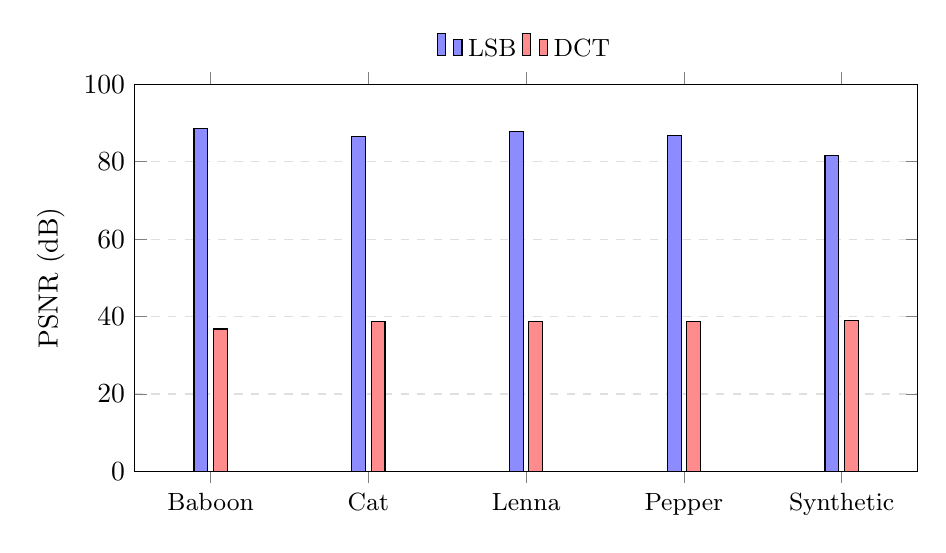
\begin{tikzpicture}
\begin{axis}[
  ybar, bar width=5pt,
  width=0.95\linewidth, height=6.5cm,
  ylabel={PSNR (dB)},
  ymin=0, ymax=100,
  symbolic x coords={Baboon,Cat,Lenna,Pepper,Synthetic},
  xtick=data, x tick label style={font=\small},
  legend style={at={(0.5,1.03)}, anchor=south, legend columns=2,
                font=\small, draw=none},
  enlarge x limits=0.12,
  ymajorgrids=true, grid style=dashed, grid style={gray!25}
]
\addplot[fill=blue!45] coordinates
  {(Baboon,88.48) (Cat,86.52) (Lenna,87.69) (Pepper,86.81) (Synthetic,81.57)};
\addplot[fill=red!45] coordinates
  {(Baboon,36.80) (Cat,38.76) (Lenna,38.71) (Pepper,38.71) (Synthetic,38.91)};
\legend{LSB, DCT}
\end{axis}
\end{tikzpicture}
\Description{Bar chart of PSNR in dB for LSB and DCT embedding across Baboon,
Cat, Lenna, Pepper, and a synthetic cover.}
\caption{PSNR (dB) as a function of embedding domain and cover image. LSB
achieves approximately $82$--$88~\mathrm{dB}$, whereas DCT achieves
approximately $37$--$39~\mathrm{dB}$.}
\label{fig:psnr}
\end{figure}

\begin{table}[t]
\centering
\small
\setlength{\tabcolsep}{4pt}
\caption{Image fidelity for LSB and DCT embedding.}
\label{tab:fidelity}
\begin{tabular}{lcccccc}
\toprule
Image & Size & MSE (LSB) & PSNR (LSB) & MSE (DCT) & PSNR (DCT)\\
\midrule
Baboon   & $515\times512$ & $0.00009$ & $88.48$ & $13.59$ & $36.80$\\
Cat      & $483\times395$ & $0.00015$ & $86.52$ & $8.66$  & $38.76$\\
Lenna    & $512\times512$ & $0.00011$ & $87.69$ & $8.75$  & $38.71$\\
Pepper   & $512\times384$ & $0.00014$ & $86.81$ & $8.74$  & $38.71$\\
Synthetic& $256\times256$ & $0.00045$ & $81.57$ & $8.35$  & $38.91$\\
\bottomrule
\end{tabular}
\end{table}

\subsection{Audio and Non-Binary Secrets}

Audio LSB embedding of eight $128$-bit shares into a one-second 16-bit PCM WAV
produced an average MSE of $0.0083$ (range across runs $0.0029$--$0.0083$), with
extracted bits identical to the embedded bits for every share and exact secret
reconstruction. For a non-binary bank code (\texttt{15467-9812}, $80$~bits,
split into ten $8$-bit blocks), block-wise generation and reconstruction
recovered the original code exactly with $k = 6$ shares, while $5$ shares
yielded no reconstruction. Thus the construction generalized from single binary
strings to arbitrary multi-block payloads without loss.

%% ===========================================================================
\section{Discussion}
\label{sec:discussion}
%% ===========================================================================

\subsection{Interpretation of Key Findings}

The central finding is that a lattice-based threshold construction and
steganographic share transport are mutually compatible: exact secret
reconstruction was preserved across all thresholds and embedding domains, while
cover fidelity remained high. Two observations merit emphasis. First, the wide
decryption margin (residual $\le 33$ versus a rounding threshold of $3{,}072$)
explains the robustness of reconstruction: even when a steganographic channel
introduces small perturbations, the rounding step in Eq.~\eqref{eq:dec} is
unaffected provided the extracted share bits are exact, which they were.
Second, the pronounced fidelity gap between LSB and DCT (roughly
$87~\mathrm{dB}$ versus $38~\mathrm{dB}$) is structural rather than
implementation-specific: LSB changes at most a handful of channel values by
$\pm1$, whereas DCT redistributes a fixed-magnitude spectral perturbation over
an entire block.

\subsection{Comparison with Existing Literature}

The cryptographic construction aligns with threshold and distributed-decryption
approaches to lattice cryptography
\cite{bendlin2010,desmedt1994,gemmell1997}, and with the LWE encryption
template of Regev \cite{regev2005} and its worst-case-to-average-case
foundations \cite{peikert2009,micciancio2009}. It differs from purely
information-theoretic sharing \cite{shamir1979,blakley1979} by wrapping the
shared key in an LWE envelope whose public transcript is protected by the LWE
assumption, itself believed hard for quantum adversaries and standardized in
the NIST PQC process \cite{nist2024,avanzi2020}. On the steganographic side,
the LSB and DCT results are consistent with classical observations that spatial
LSB substitution maximizes imperceptibility \cite{chan2004,bender1996} whereas
frequency-domain methods trade fidelity for robustness \cite{westfeld2001,fridrich2009}.
The novelty relative to prior counting-based prototypes is the substitution of
a post-quantum sharing primitive and the accompanying quantitative
characterization of the resulting pipeline.

An important conceptual clarification concerns the locus of security. The
share \emph{distribution} relies on Shamir's information-theoretic
security---already quantum-proof---while the \emph{public transcript} (the
matrix $\mathbf{A}$, the vector $\mathbf{b}$, and the ciphertexts) relies on
LWE. Thus an adversary holding fewer than $k$ shares learns nothing about the
key from the shares themselves and cannot recover it from the public transcript
without solving LWE. This layered argument is what justifies the
``post-quantum'' characterization; it should not be read as a claim that the
threshold structure itself derives hardness from lattices.

\subsection{Limitations of the Study}

Several limitations constrain the conclusions. First, the parameter set
($q = 12{,}289$, $n = 8$, $m = 32$) is intentionally small for demonstration and
does not meet production security targets; the reported timings and payload
sizes therefore do not extrapolate to secure parameters. Second, the study is
an empirical characterization, not a formal cryptographic analysis: no
reduction from the scheme's security to a worst-case lattice problem is proved,
and no concrete security estimate (e.g., via the lattice-estimator methodology)
is provided. Third, steganographic security was assessed only through
image-fidelity metrics (MSE/PSNR); no steganalysis resistance was measured, so
robustness to statistical detectors \cite{westfeld2001,fridrich2009} is
unknown. Fourth, the audio evaluation used a single synthetic tone; natural
audio and compression (e.g., MP3) were not examined, and the DCT method is
fragile to recompression and cropping. Fifth, the current model shares the LWE
secret key and publishes ciphertexts; multi-secret key reuse and adaptive
corruption were not analyzed. Finally, the reference implementation is a
prototype, not an audited library.

\subsection{Implications and Future Directions}

Notwithstanding these caveats, the results suggest a practical pathway for
quantum-resistant distributed trust with covert share transport: organizations
can layer steganographic transport atop post-quantum threshold primitives
without sacrificing reconstruction integrity, choosing the embedding domain
according to the robustness--imperceptibility trade-off. Future work should
proceed along five axes: (i) scale to conservative post-quantum parameters and
provide concrete security estimates; (ii) formulate and, where possible, prove
a reduction for the composed scheme; (iii) evaluate steganalysis resistance,
including RS and DCT-histogram detectors, and adopt encoding with error
correction for robustness to compression; (iv) extend to verifiable and
proactive (key-refreshing) sharing, and to malicious-participant models; and
(v) investigate secret sharing directly over the ring
$\mathbb{Z}_q[X]/(X^N+1)$ (Ring-LWE) to reduce share size and enable efficient,
threshold-friendly arithmetic.

%% ===========================================================================
\section{Conclusion}
\label{sec:conclusion}
%% ===========================================================================

This paper presented an integrated, post-quantum threshold secret sharing
construction in which a Regev-style LWE secret key is shared over
$\mathbb{Z}_q$ via Shamir's scheme and each participant's share is concealed
using spatial, frequency-domain, or audio steganography. A reference
implementation confirmed exact reconstruction for all thresholds tested,
correct refusal below threshold, and high cover fidelity---PSNR of
$81.6$--$88.5~\mathrm{dB}$ for LSB and $36.8$--$38.8~\mathrm{dB}$ for DCT, with
audio LSB MSE on the order of $10^{-3}$. The principal takeaway is that
post-quantum threshold sharing and covert share transport can coexist without
compromising secret integrity, and that the choice of embedding domain governs
a clear fidelity--robustness trade-off. Because the present parameters are
demonstrative and the analysis empirical, the work should be regarded as a
proof of feasibility and a scaffold for the security-theoretic and steganalytic
evaluations that a deployable system will require.

%% ===========================================================================
\section*{CRediT authorship contribution statement}
%% ===========================================================================
\textbf{Franklin Lenny TADMON-YAYA:} Conceptualization, Methodology, Software,
Validation, Formal analysis, Investigation, Writing -- original draft, Writing
-- review \& editing, Supervision.

%% ===========================================================================
\section*{Data availability}
%% ===========================================================================
The source code, parameter set, embedding routines, and benchmark harness that
support the findings of this study are publicly available at
\url{https://github.com/tadmonyayafranklin-netizen/LatticeStegoShare}. The
standard test images (Baboon, Cat, Lenna, Pepper) are publicly available.

\begin{credits}
\subsubsection{\ackname} The authors thank the members of the
information-security research group for valuable discussions and for providing
computational resources. This research received no specific grant from any
funding agency in the public, commercial, or not-for-profit sectors.

\subsubsection{\discintname}
The authors have no competing interests to declare that are relevant to the
content of this article.
\end{credits}

%% ===========================================================================
% ---- Bibliography ----
%% ===========================================================================
\bibliographystyle{splncs04}
\bibliography{refs}

\end{document}
